\documentclass[journal,onecolumn,11pt]{IEEEtran}
\usepackage[T1]{fontenc}
\usepackage{amsmath,amssymb}
\usepackage{graphicx}
\usepackage{booktabs}
\usepackage{array}
\usepackage{tabularx}
\usepackage{algorithm}
\usepackage[noend]{algpseudocode}
\usepackage{cite}
\usepackage{xcolor}
\usepackage[hidelinks]{hyperref}
\usepackage{float}
\renewcommand{\arraystretch}{1.12}
\newcolumntype{L}{>{\raggedright\arraybackslash}X}

\begin{document}
\title{Reproducing and Extending the MTTD Dynamic Model-Selection Framework: Five ML Models on a 2023 Cricket World Cup Workload with CloudSim Evaluation}

\author{Abhinav~Mishra, Garv~Gujral, and~Shashank~Yadav%
\thanks{The authors are with Netaji Subhas University of Technology, New Delhi 110075, India.}%
\thanks{Code, workload generator and simulation: \url{https://github.com/garv-codes/ML-workload-prediction}.}}

\markboth{Preprint, November 2026}{Reproducing and Extending MTTD on a Cricket World Cup Workload}
\maketitle

\begin{abstract}
Nashaat \emph{et al.} (2026) proposed MTTD, a Monitor--Train--Test--Deploy framework that trains several workload predictors, deploys the one with the lowest error score, and retrains when an adaptive threshold is breached on two consecutive cycles. They evaluated three models (ARIMA, SVR, Random Forest) on FIFA World Cup server logs. We reproduce the framework with five models, adding XGBoost and an LSTM, and apply it to an hourly workload derived from daily Wikipedia page views (user traffic) of the 2023 ICC Cricket World Cup. We also add an option that re-selects the active model every day or every hour, and replay every forecast in a CloudSim data-centre simulation. In the standard MTTD run, the test phase selected Random Forest (Score 6.49\%), one retraining event re-selected it, and it remained active for all 1,080 deployment hours (Score 32.78\%), although the best-scoring model varied from day to day. Re-selecting every day or every hour made the active model switch 27 and 77 times and lowered the score to 21.41\% and 18.96\%. In CloudSim 3.0.3, standard MTTD provisioned 7,475 VM-hours against 6,981 needed and violated the SLA in 145 of 1,080 hours; hourly reselection reduced wasted VM-hours from 1,077 to 702 but raised SLA-violating hours to 158, and daily reselection to 263.
\end{abstract}

\begin{IEEEkeywords}
Cloud autoscaling, workload prediction, dynamic model selection, concept drift, flash crowds, CloudSim, XGBoost, LSTM.
\end{IEEEkeywords}

\section{Introduction}
\IEEEPARstart{E}{lastic} cloud platforms promise capacity that tracks demand, but the controllers that deliver it are mostly reactive. A threshold autoscaler, such as the Kubernetes Horizontal Pod Autoscaler~\cite{k8shpa}, adds replicas only after utilisation has already crossed a target, so the first minutes of a surge are served by an undersized fleet~\cite{lorido2014,qu2018,herbst2013}. Production systems at hyperscale therefore combine reactive control with forecasting~\cite{rzadca2020,verma2015}.

Live sports events are a hard case for forecasting. Audience attention concentrates in match windows, swings between fixtures of different importance, and peaks during knockout games and finals. Such flash crowds are well documented for web workloads since the 1998 FIFA World Cup~\cite{arlitt2000,jung2002}. A forecaster trained on the group stage sees a different distribution from the one it must serve during the semi-finals, an instance of concept drift~\cite{gama2014}.

Comparative studies repeatedly find that no single model dominates across workload patterns~\cite{calheiros2015,kim2016,liu2017,cetinski2015}. Nashaat \emph{et al.}~\cite{nashaat2026} responded with MTTD, a Monitor--Train--Test--Deploy loop that trains several candidates, deploys the best, and retrains when an error-amplified threshold is breached on two consecutive cycles. Their evaluation used the 1998 and 2018 FIFA World Cup server logs and three candidates (ARIMA, SVR, Random Forest), and stopped at prediction accuracy.

This paper reproduces MTTD and extends it. Its contributions are:
\begin{enumerate}
\item \textbf{Reproduction of the MTTD pipeline.} We implement all four phases of~\cite{nashaat2026}, including its performance score and two-strike adaptive retraining threshold, and repeat its synthetic-workload experiments.
\item \textbf{Five candidate models.} We add gradient boosting (XGBoost~\cite{chen2016}) and a recurrent network (LSTM~\cite{hochreiter1997}) to the original ARIMA, SVR and Random Forest candidates.
\item \textbf{A 2023 Cricket World Cup workload.} In place of the FIFA logs, we disaggregate 56 daily English-Wikipedia page-view counts (user traffic) for the tournament article into 1,344 hourly intervals.
\item \textbf{Periodic reselection.} We add an option that re-chooses the active model every $N$ hours from its recent error, and run it with $N=24$ (daily) and $N=1$ (hourly).
\item \textbf{CloudSim evaluation.} Every run's hourly forecasts are replayed in a CloudSim~\cite{calheiros2011} data-centre simulation that provisions VMs from the forecast and executes the real load.
\end{enumerate}
Section~\ref{sec:related} reviews related work. Section~\ref{sec:method} presents the method. Section~\ref{sec:results} reports the experimental setup and results. Section~\ref{sec:conclusion} concludes.

\section{Related Work}\label{sec:related}
Workload prediction for autoscaling has been surveyed extensively~\cite{lorido2014,qu2018,amiri2017,masdari2020}. We group prior work into four families, summarised in Fig.~\ref{fig:taxonomy} and Table~\ref{tab:related}.

\begin{figure}[H]
\centering
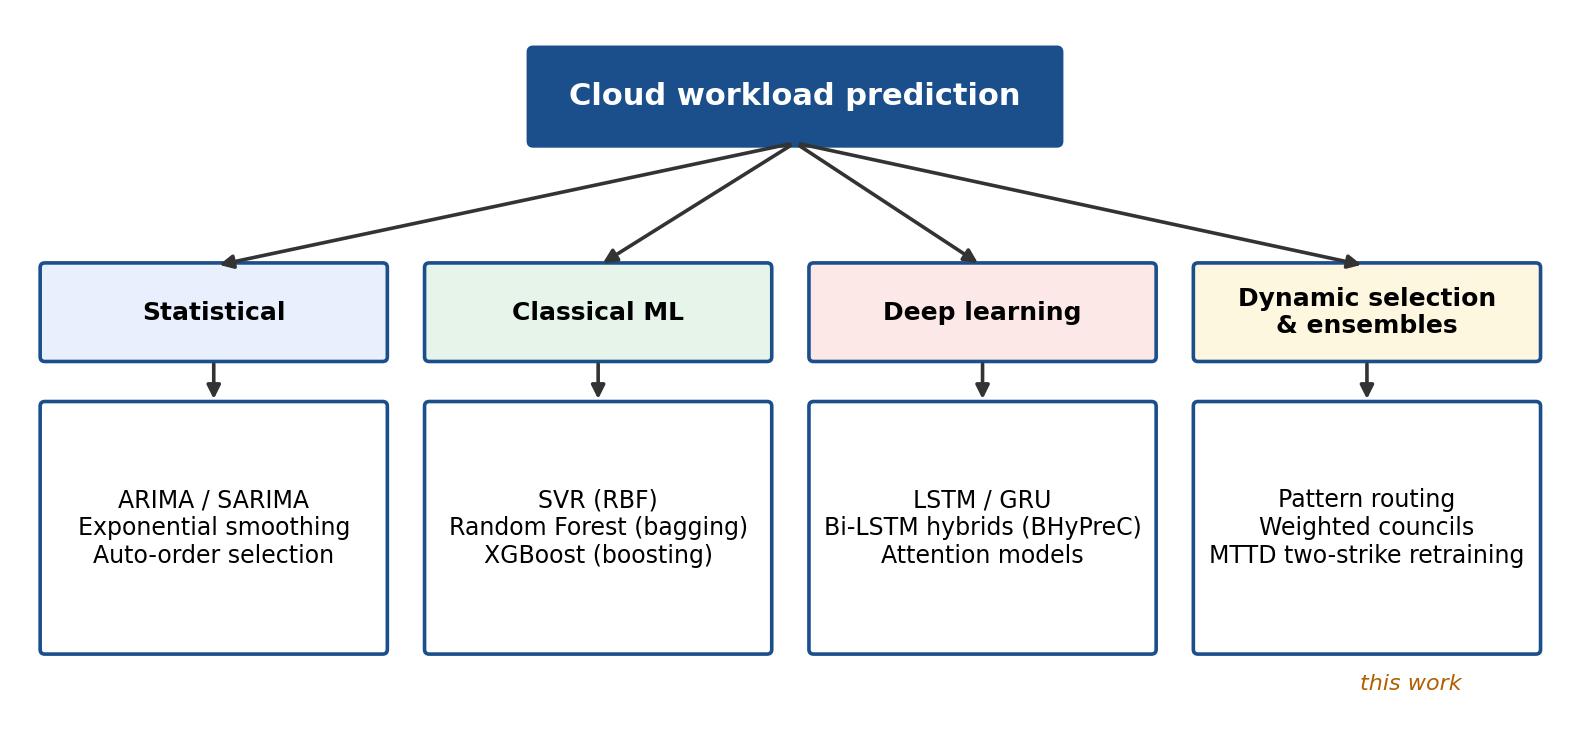
\includegraphics[width=0.82\linewidth]{fig1_taxonomy.png}
\caption{Taxonomy of cloud workload prediction approaches. This work extends the dynamic-selection family.}
\label{fig:taxonomy}
\end{figure}

\subsection{Statistical Models}
ARIMA models a series through autoregressive, differencing and moving-average terms~\cite{box2015}. Calheiros \emph{et al.}~\cite{calheiros2015} used ARIMA to forecast web requests and evaluated its effect on QoS in CloudSim. Automatic order selection~\cite{hyndman2008} removes manual ACF/PACF tuning. Early predictive scalers such as PRESS~\cite{gong2010} and CloudScale~\cite{shen2011} paired signal-processing or Markov predictors with corrective control. ARIMA assumes linear, locally stationary dynamics, so strong intraday seasonality degrades it unless a seasonal term is modelled.

\subsection{Classical Machine Learning}
Support vector regression~\cite{drucker1997} and Random Forests~\cite{breiman2001} recast forecasting as supervised regression on a sliding window of lags. Empirical comparisons~\cite{islam2012,kim2016} evaluated such learners against time-series models, and Kim \emph{et al.}~\cite{kim2016} found that no single predictor is best for all workload patterns. Later studies applied these learners directly to elastic provisioning~\cite{gao2020,moreno2019}. Gradient boosting with XGBoost~\cite{chen2016} adds shrinkage and regularised tree growth.

\subsection{Deep Learning}
LSTMs~\cite{hochreiter1997} capture long-range temporal dependence through gated memory. Kumar and Singh~\cite{kumar2018,kumar2021} trained neural forecasters with evolutionary and self-directed learning. Bi \emph{et al.}~\cite{bi2021} combined bidirectional and grid LSTMs (BG-LSTM). BHyPreC~\cite{karim2021} stacks Bi-LSTM, LSTM and GRU layers for VM CPU prediction.

\subsection{Dynamic Selection and Ensembles}
Because no single model dominates, several works select or combine models online. Liu \emph{et al.}~\cite{liu2017} discriminate workload patterns and route each to a matching predictor. AME-WPC~\cite{cetinski2015} combines several forecasting methods, and Messias \emph{et al.}~\cite{messias2016} combine time-series models with a genetic algorithm. CloudInsight~\cite{kim2022} maintains a council of predictors and reweights them over time. MTTD~\cite{nashaat2026} instead deploys one active model and retrains all candidates only when an error-amplified threshold is breached twice in a row.

\begin{table}[H]
\centering
\caption{Representative Workload-Prediction Approaches}
\label{tab:related}
\footnotesize
\begin{tabularx}{\linewidth}{@{}l L l l L@{}}
\toprule
Ref. & Approach & Family & Dynamic selection & Evaluation scope\\
\midrule
\cite{calheiros2015} & ARIMA & Statistical & No & Forecast accuracy and QoS impact in CloudSim\\
\cite{roy2011} & ARMA + look-ahead control & Statistical & No & Forecasting with autoscaling control\\
\cite{islam2012} & NN, linear regression & Classical ML & No & Forecast accuracy\\
\cite{kim2016} & 21 predictors compared & Mixed & No & 24 synthetic workloads; cost and deadline-miss simulation\\
\cite{kumar2018} & NN + adaptive DE & Deep / evolutionary & No & Forecast accuracy\\
\cite{karim2021} & Bi-LSTM + LSTM + GRU (BHyPreC) & Deep learning & No & VM CPU forecast accuracy\\
\cite{liu2017} & Pattern-routed predictors & Dynamic & Yes (by pattern) & Forecast accuracy vs.\ ARIMA, SVM, LR\\
\cite{kim2022} & Predictor council (CloudInsight) & Ensemble & Yes (reweighting) & Real traces; trace-based provisioning simulation\\
\cite{nashaat2026} & MTTD: ARIMA, SVR, RF & Dynamic & Yes (two-strike) & Forecast accuracy on FIFA 1998 and 2018 logs\\
This work & MTTD: + XGBoost, LSTM & Dynamic & Yes (two-strike; periodic) & Forecast accuracy and CloudSim provisioning\\
\bottomrule
\end{tabularx}
\end{table}

This work follows~\cite{nashaat2026} and adds two models, a new workload, periodic model reselection and a CloudSim provisioning evaluation (last row of Table~\ref{tab:related}).

\section{Methodology}\label{sec:method}

\subsection{Two-Stage Pipeline}
The system separates prediction from provisioning (Fig.~\ref{fig:arch}). Stage~1, in Python (\texttt{mttd\_bridge.py}), runs the online MTTD loop over the hourly trace and writes, for every deployment hour, the observed load, the active model's one-step-ahead forecast, the active model's name and any retraining event to a CSV file. Stage~2, in Java (\texttt{ProvisioningSimulation.java}), reads that file and replays each hour in CloudSim.

\begin{figure}[H]
\centering
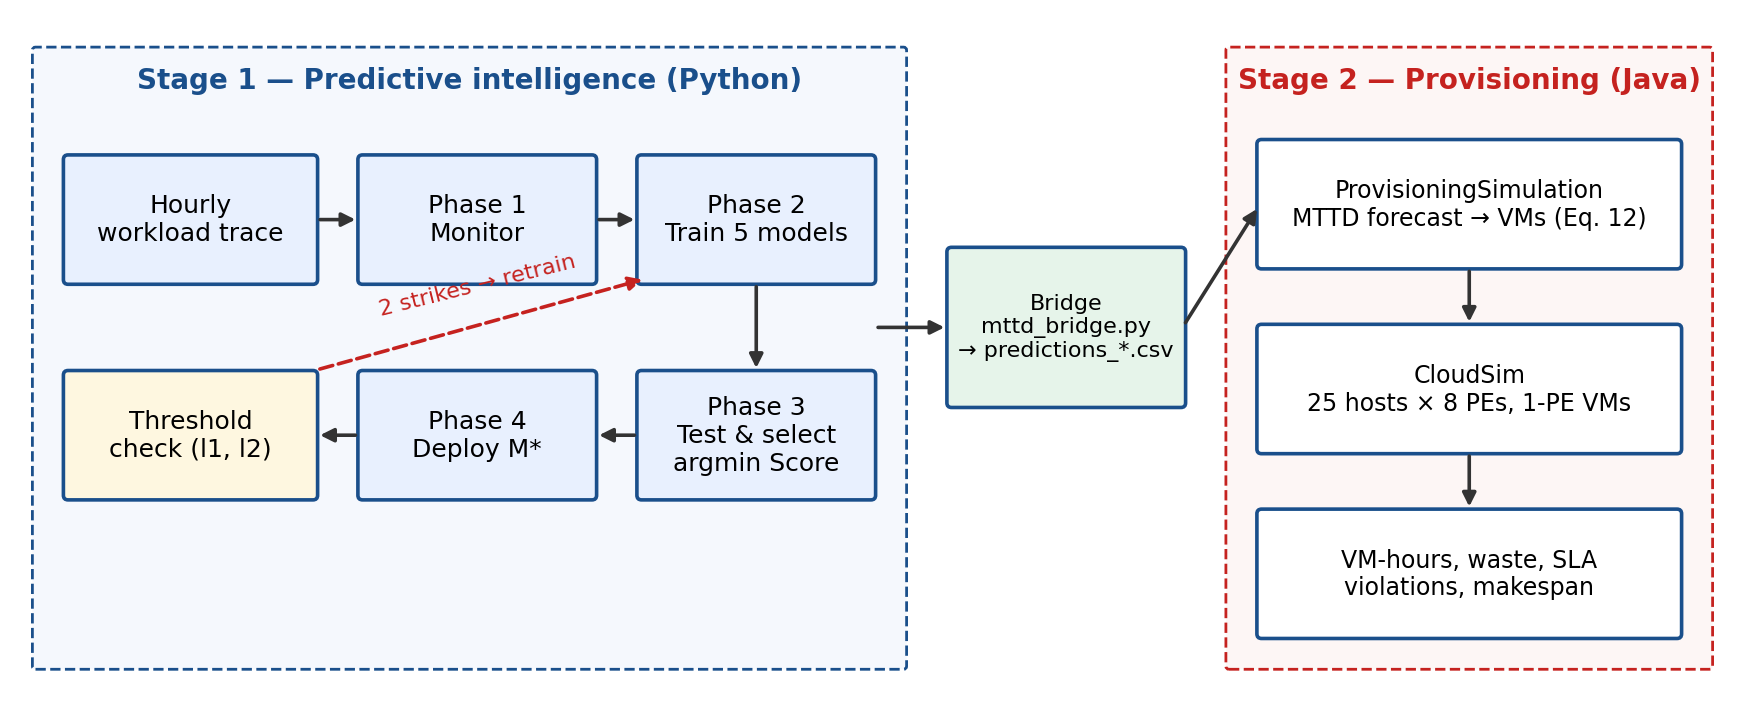
\includegraphics[width=0.9\linewidth]{fig2_architecture.png}
\caption{Two-stage pipeline: the Python MTTD loop (Stage 1), the CSV file of hourly forecasts, and the Java CloudSim simulation (Stage 2).}
\label{fig:arch}
\end{figure}

\subsection{Metrics}
Let $y_t$ be the number of requests in hour $t$ and $\hat{y}^{(i)}_t$ the one-step-ahead forecast of candidate $i\in\mathcal{M}=\{\text{ARIMA},\text{SVR},\text{RF},\text{XGB},\text{LSTM}\}$, made from observations up to $t-1$. Over an evaluation window of $N$ hours we use the error measures of~\cite{nashaat2026,hyndman2006}:
\begin{align}
\mathrm{RMSE}_i &= \sqrt{\tfrac{1}{N}\textstyle\sum_{t=1}^{N}\big(y_t-\hat{y}^{(i)}_t\big)^2},\\
\mathrm{MAE}_i &= \tfrac{1}{N}\textstyle\sum_{t=1}^{N}\big|y_t-\hat{y}^{(i)}_t\big|.
\end{align}
MTTD ranks models by the normalised, weighted score of~\cite{nashaat2026} (its Eq.~4) with $w_1=w_2=0.5$:
\begin{equation}
\mathrm{Score}_i = 100\left(w_1\frac{\mathrm{RMSE}_i}{\sqrt{\frac{1}{N}\sum_t y_t^2}}+w_2\frac{\mathrm{MAE}_i}{\frac{1}{N}\sum_t y_t}\right).
\end{equation}
The active model is the candidate with the lowest score on the test window:
\begin{equation}
M^{*}=\arg\min_{i\in\mathcal{M}}\mathrm{Score}_i .
\end{equation}
On the synthetic benchmarks we also report $\mathrm{MAPE}_i=\frac{100}{N}\sum_t |y_t-\hat{y}^{(i)}_t|/|y_t|$.

\subsection{Two-Strike Retraining Threshold}
The active model is deployed for cycles of 24 hours. Let $S_t$ be its score on cycle $t$. Following~\cite{nashaat2026}, the threshold for the next cycle is set from the latest healthy score with weight $l_1$, and set with weight $l_2$ after a first breach:
\begin{align}
\mathrm{Threshold}_{t+1} &= S_t + l_1 S_t, & l_1&=0.75,\\
\mathrm{Threshold}_{t+2} &= S_{t+1} + l_2 S_{t+1}, & l_2&=0.50.
\end{align}
A strike counter $k$ implements the two-strike rule, retraining at $t$ if and only if $k_t=2$:
\begin{equation}
k_t=\begin{cases}0, & S_t\le \mathrm{Threshold}_t,\\ k_{t-1}+1, & S_t>\mathrm{Threshold}_t.\end{cases}
\end{equation}
On retraining, all five candidates are refitted on the latest 240 hours, re-tested on the last 24 hours, and the lowest-scoring model becomes active. Algorithm~\ref{alg:mttd} and Fig.~\ref{fig:flow} summarise the loop. All candidates forecast every hour so that their scores can be logged, but only the active model's forecasts are written to the output file.

\begin{algorithm}[H]
\caption{Online MTTD with two-strike retraining}
\label{alg:mttd}
\small
\begin{algorithmic}[1]
\Require series $y$, candidates $\mathcal{M}$, $T_{tr}{=}240$\,h, $T_{te}{=}24$\,h, cycle $n{=}24$\,h, window $w{=}24$, $l_1{=}0.75$, $l_2{=}0.50$
\State $t\gets T_{tr}+T_{te}$ \Comment{Phase 1: monitor}
\State fit every $m\in\mathcal{M}$ on $y[t{-}T_{tr}{-}T_{te}:t{-}T_{te}]$ \Comment{Phase 2}
\State $S_m\gets$ Score of rolling forecast of $y[t{-}T_{te}:t]$ for all $m$
\State $M^*\gets\arg\min_m S_m$;\ $\theta\gets S_{M^*}(1{+}l_1)$;\ $k\gets0$ \Comment{Phase 3}
\While{$t<|y|$} \Comment{Phase 4: deploy}
  \State forecast $y[t:t{+}n]$ one step ahead with $M^*$, observing truth
  \State $S\gets$ Score of this cycle
  \If{$S\le\theta$} \State $k\gets0$;\ $\theta\gets S(1{+}l_1)$
  \Else \State $k\gets k+1$
    \If{$k=1$} \State $\theta\gets S(1{+}l_2)$
    \Else \State $k\gets0$;\ $t'\gets t+n$
      \State refit all $m$ on $y[t'{-}T_{tr}{-}T_{te}:t'{-}T_{te}]$
      \State re-test on $y[t'{-}T_{te}:t']$;\ $M^*\gets\arg\min$;\ $\theta\gets S_{M^*}(1{+}l_1)$
    \EndIf
  \EndIf
  \State $t\gets t+n$
\EndWhile
\end{algorithmic}
\end{algorithm}

\begin{figure}[H]
\centering
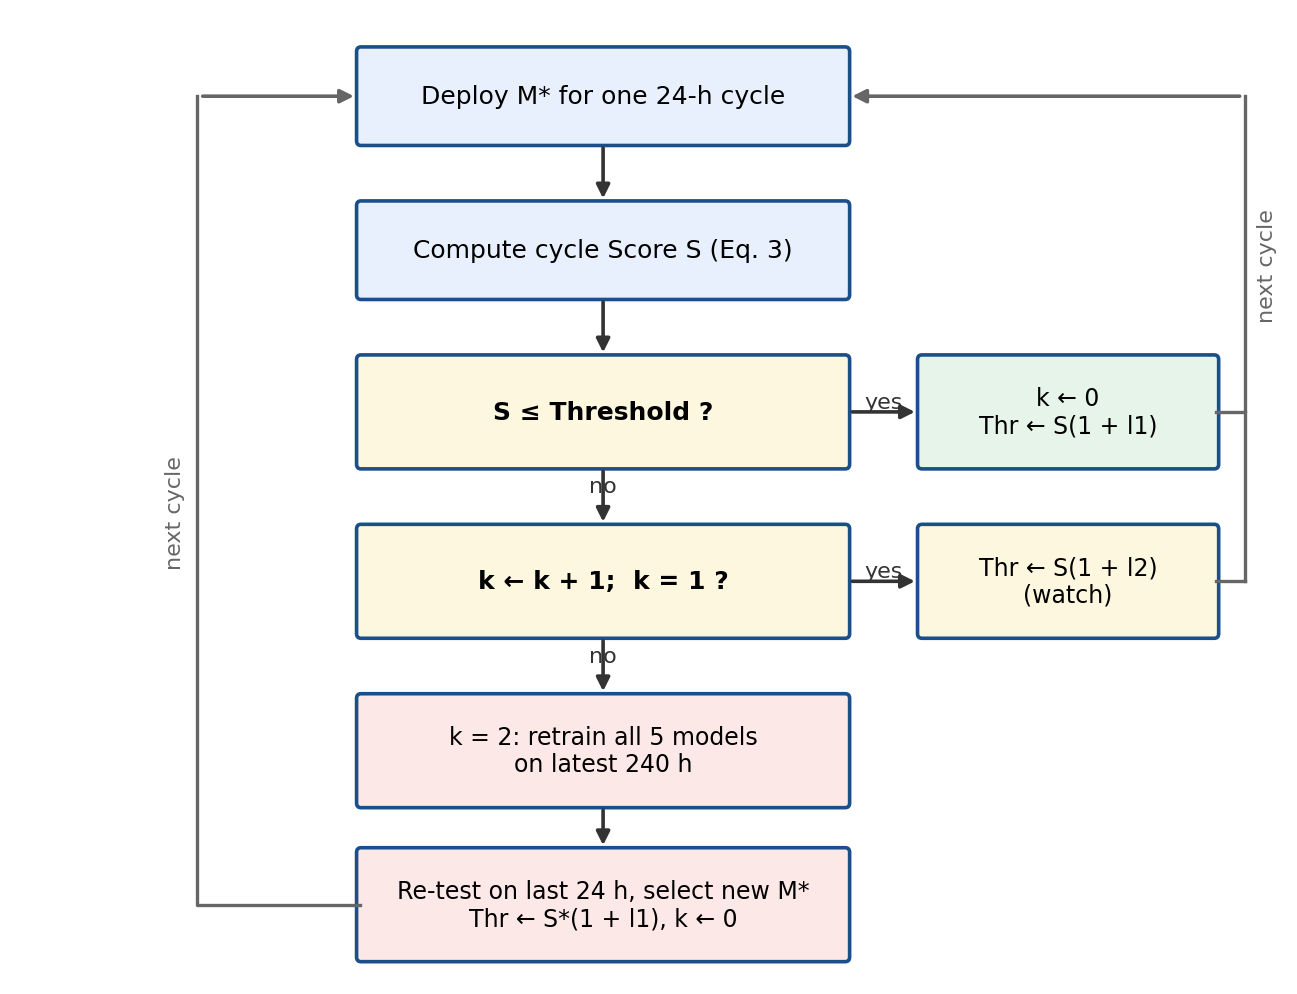
\includegraphics[width=0.62\linewidth]{fig3_flowchart.png}
\caption{Retraining and model-reselection flowchart implementing Eqs.~(5)--(7).}
\label{fig:flow}
\end{figure}

\subsection{Data Engineering: Daily-to-Hourly Disaggregation}
Daily page views $D_d$ for the English Wikipedia article ``2023 Cricket World Cup'' were exported from the Wikimedia Pageviews tool~\cite{wikimedia} for 1~Oct--25~Nov 2023 (56 days) with agent = user, which excludes bots and automated traffic. Let $h\in\{0,\dots,23\}$ be the hour of day. The match window $\mathcal{P}=\{14,\dots,21\}$ receives 70\% of the day's traffic and the 16 other hours share 30\%:
\begin{equation}
b_{d,h}=\begin{cases}0.70\,D_d/8, & h\in\mathcal{P},\\ 0.30\,D_d/16, & h\notin\mathcal{P}.\end{cases}
\end{equation}
Each hour is perturbed by bounded uniform noise:
\begin{equation}
\tilde{y}_{d,h}=b_{d,h}\,\varepsilon_{d,h},\qquad \varepsilon_{d,h}\sim\mathcal{U}(0.92,\,1.08).
\end{equation}
The noisy hours are renormalised so that each day keeps its real total, and rounded with the residual assigned to the largest hour:
\begin{equation}
y_{d,h}=\mathrm{round}\!\left(\tilde{y}_{d,h}\,\frac{D_d}{\sum_{h'}\tilde{y}_{d,h'}}\right),\qquad \sum_h y_{d,h}=D_d .
\end{equation}
A fixed random seed (42) makes the trace reproducible.

\subsection{Periodic Reselection (Extension)}
In standard MTTD the active model changes only at a retraining event. As an extension, \texttt{mttd\_bridge.py} accepts an option \texttt{--reselect-every}~$N$: every $N$ hours the active model is replaced by the candidate with the lowest score over the most recent $W=24$ hours of logged forecasts,
\begin{equation}
M^{*}_t=\arg\min_{i\in\mathcal{M}}\mathrm{Score}_i\big(y_{t-W:t},\,\hat{y}^{(i)}_{t-W:t}\big),\qquad t \equiv t_0 \pmod N .
\end{equation}
The two-strike retraining rule stays active and is evaluated on the forecasts actually used. We run $N=24$ (daily) and $N=1$ (hourly).

\subsection{CloudSim Provisioning Model}
For each hour, the number of VMs is set from the forecast with headroom $\eta=1.10$ and a cap of $V_{\max}=150$:
\begin{equation}
V_t=\min\!\big(V_{\max},\max(1,\lceil \eta\,\hat{y}_t/C\rceil)\big),
\end{equation}
where $C=4{,}000$ is the number of requests one VM serves per hour (900~MI per request on a 1,000-MIPS VM). The VMs needed if the load were known exactly are
\begin{equation}
V^{\mathrm{req}}_t=\min\!\big(V_{\max},\max(1,\lceil y_t/C\rceil)\big).
\end{equation}
The hour's real requests are executed in CloudSim as cloudlets of 200 requests (180,000~MI, 180~s on one VM), assigned round-robin to time-shared VMs. An hour violates the SLA if the last cloudlet finishes after one hour:
\begin{equation}
\mathrm{SLA}_t=\mathbb{1}\big[T_t>3600\,\mathrm{s}\big].
\end{equation}
We report VM-hours provisioned and needed, wasted VM-hours ($\sum_t\max(0,V_t-V^{\mathrm{req}}_t)$), under-provisioned hours ($V_t<V^{\mathrm{req}}_t$), SLA-violating hours and the average completion time.

\section{Experimental Setup and Results}\label{sec:results}

\subsection{Setup}
Table~\ref{tab:sim} lists the CloudSim parameters and Table~\ref{tab:hyper} the candidate models. All window-based models use the last 24 hourly values as features; the training window is 240 hours, the test window 24 hours and the deployment cycle 24 hours, matching the hourly configuration of~\cite{nashaat2026}. Grid searches use 3-fold \texttt{GridSearchCV} with negative MSE~\cite{pedregosa2011}; the LSTM uses PyTorch~\cite{paszke2019}.

\begin{table}[H]
\centering
\caption{CloudSim Simulation Parameters (\texttt{ProvisioningSimulation.java}, CloudSim 3.0.3)}
\label{tab:sim}
\footnotesize
\begin{tabularx}{\linewidth}{@{}l L@{}}
\toprule
Parameter & Value\\
\midrule
Data centre & 25 hosts $\times$ 8 PEs $\times$ 1,000 MIPS, 16 GB RAM, time-shared VM scheduler\\
VM & 1 PE, 1,000 MIPS, 512 MB RAM, time-shared cloudlet scheduler\\
Capacity $C$ & 4,000 requests per VM per hour (900 MI per request)\\
Cloudlet & 200 requests = 180,000 MI (180 s on one VM)\\
Headroom $\eta$ / cap $V_{\max}$ & 1.10 / 150 VMs\\
Time step and SLA & 3,600 s; all cloudlets of the hour must finish within 3,600 s\\
Horizon & 1,080 hours (hours 264--1343)\\
Software & CloudSim 3.0.3, JDK 26\\
\bottomrule
\end{tabularx}
\end{table}

\begin{table}[H]
\centering
\caption{Candidate Predictors on the Cricket Trace (\texttt{mttd\_bridge.py})}
\label{tab:hyper}
\footnotesize
\begin{tabularx}{\linewidth}{@{}l L@{}}
\toprule
Model & Configuration and search grid\\
\midrule
ARIMA & \texttt{pmdarima.auto\_arima}~\cite{hyndman2008}, non-seasonal, $p,q\le5$, $d$ by unit-root test, stepwise; updated with each new observation\\
SVR & RBF; $C\in\{1,10,100\}$, $\epsilon\in\{0.001,0.01\}$, $\gamma\in\{0.01,0.1\}$; inputs scaled by the training maximum\\
Random Forest & 100 trees; max depth $\in\{10,40\}$; min samples/leaf $\in\{1,3\}$\\
XGBoost & trees $\in\{100,200\}$; max depth $\in\{3,6\}$; learning rate $\in\{0.05,0.1\}$\\
LSTM & 1 layer $\times$ 32 units + linear head; Adam, lr 0.01; 60 epochs; batch 32; z-score inputs; seed 42\\
\bottomrule
\end{tabularx}
\end{table}

\subsection{Dataset Characteristics}
Table~\ref{tab:data} summarises the trace and Fig.~\ref{fig:workload} plots it. Within each day the trace is a two-level step with noise; across days it follows the fixture schedule, rising through the semi-finals (15--16~Nov) to the Final (19~Nov) and collapsing after the tournament (20--25~Nov, hours 1200--1343).

\begin{table}[H]
\centering
\caption{The 2023 Cricket World Cup Hourly Trace}
\label{tab:data}
\footnotesize
\begin{tabularx}{\linewidth}{@{}l L@{}}
\toprule
Property & Value\\
\midrule
Source & Wikimedia Pageviews, en.wikipedia, ``2023 Cricket World Cup'', agent = user~\cite{wikimedia}\\
Span & 1 Oct -- 25 Nov 2023; 56 days; 1,344 hourly intervals\\
Total workload & 29,957,762 requests (equal to the sum of the daily counts)\\
Deployment window & Hours 264--1343: 25,636,322 requests; mean 23,737 per hour\\
Peak & 117,612 requests at 17:00, 19 Nov 2023 (the Final; hour 1193)\\
Hourly profile & 8.75\% of daily traffic per match hour (14:00--21:00), 1.875\% per other hour; noise $\mathcal{U}(0.92,1.08)$\\
\bottomrule
\end{tabularx}
\end{table}

\begin{figure}[H]
\centering
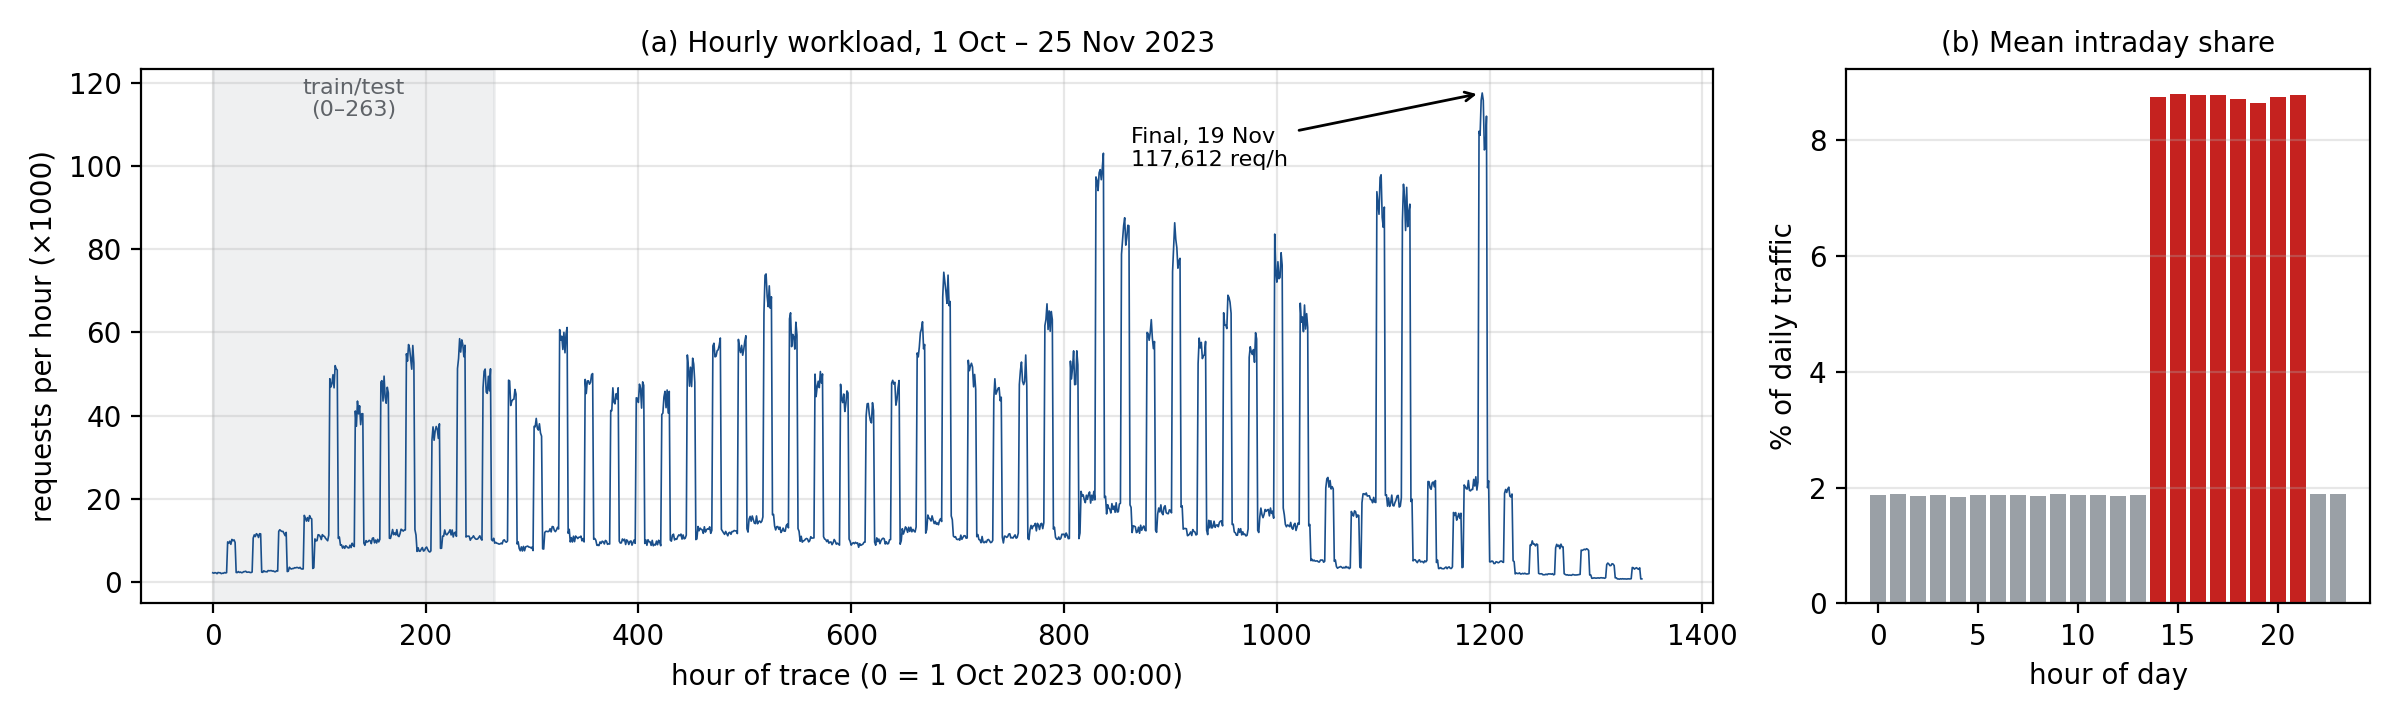
\includegraphics[width=\linewidth]{fig4_workload.png}
\caption{(a) Hourly cricket workload, 1 Oct -- 25 Nov 2023; the shaded region is the initial training and test window. (b) Mean share of daily traffic by hour of day.}
\label{fig:workload}
\end{figure}

\subsection{Synthetic Benchmark}
We ran each predictor on the four synthetic patterns of~\cite{nashaat2026} (697 minutes, 70/30 split, 100-point test window, window of 5) using \texttt{run\_benchmark.py} (Table~\ref{tab:synth}, Fig.~\ref{fig:synth}). ARIMA scored best on all four patterns. The original paper reports SVR as the best model on its random workload~\cite{nashaat2026}; in our reproduction SVR was worst on three of the four patterns.

\begin{table}[H]
\centering
\caption{Synthetic Benchmarks: Score \% (MAPE in Parentheses); Best per Pattern in Bold}
\label{tab:synth}
\footnotesize
\begin{tabular}{@{}lllll@{}}
\toprule
Model & Uniform (bell) & Linear low (0.35) & Linear high (2.31) & Bounded random walk\\
\midrule
ARIMA & \textbf{1.51 (1.42\%)} & \textbf{0.49 (0.44\%)} & \textbf{0.08 (0.07\%)} & \textbf{3.63 (3.28\%)}\\
SVR & 11.11 (11.49\%) & 50.95 (49.73\%) & 54.28 (54.05\%) & 7.73 (7.00\%)\\
Random Forest & 3.95 (3.96\%) & 10.56 (9.61\%) & 10.25 (9.29\%) & 3.96 (3.66\%)\\
XGBoost & 4.35 (4.31\%) & 10.46 (9.51\%) & 10.28 (9.32\%) & 3.83 (3.55\%)\\
LSTM & 3.70 (3.80\%) & 2.29 (2.17\%) & 2.14 (2.06\%) & 3.69 (3.40\%)\\
\bottomrule
\end{tabular}
\end{table}

\begin{figure}[H]
\centering
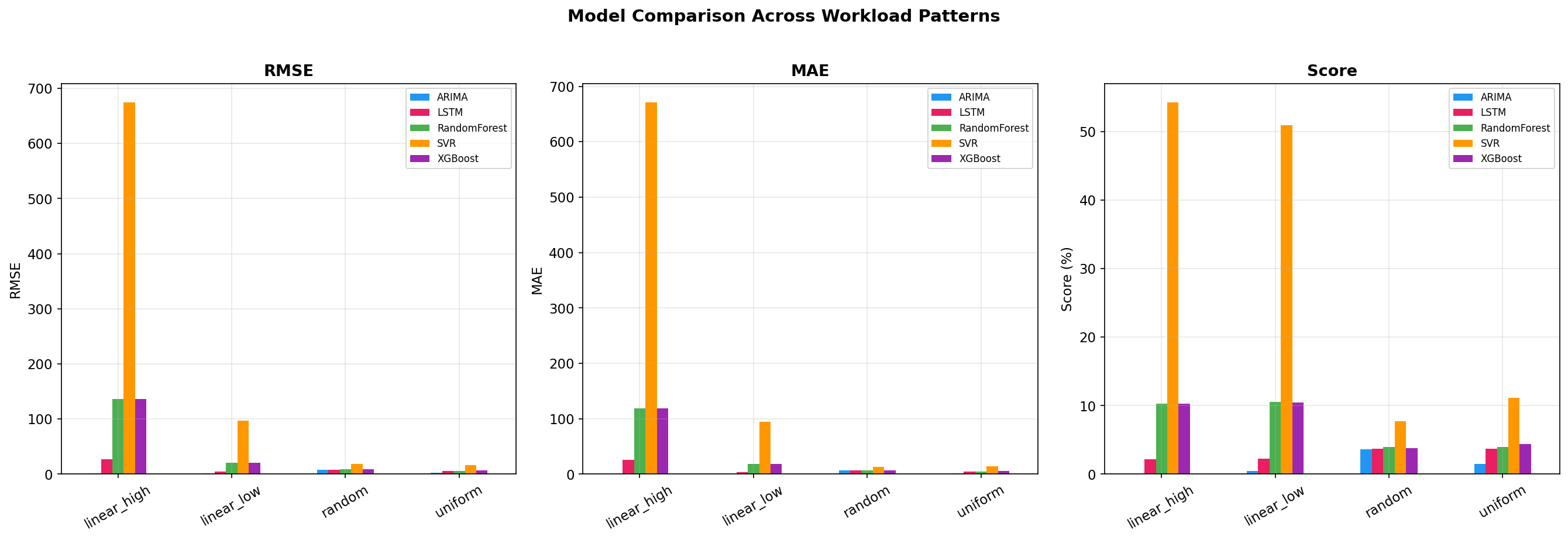
\includegraphics[width=0.95\linewidth]{fig7_synthetic.png}
\caption{RMSE, MAE and Score of the five predictors across the four synthetic workload patterns.}
\label{fig:synth}
\end{figure}

\subsection{Standard MTTD on the Cricket Trace}
The initial test window (hours 240--263) ranked Random Forest first (Table~\ref{tab:test}). One retraining event occurred, at hour 552, and the re-test again selected Random Forest, which therefore remained active for all 1,080 deployment hours.

\begin{table}[H]
\centering
\caption{Test-Phase Scores (\%) Used for Model Selection}
\label{tab:test}
\footnotesize
\begin{tabular}{@{}lrrrrrl@{}}
\toprule
Test window & RF & XGBoost & LSTM & SVR & ARIMA & Selected\\
\midrule
Initial (hours 240--263) & \textbf{6.49} & 7.07 & 7.55 & 11.75 & 29.18 & Random Forest\\
Retrain at hour 552 & \textbf{5.42} & 7.15 & 9.44 & 7.48 & 33.26 & Random Forest\\
\bottomrule
\end{tabular}
\end{table}

Table~\ref{tab:strikes} lists every threshold breach of the active model. Ten breaches produced one retraining event; eight single-cycle breaches were absorbed because the following cycle stayed below the threshold set by Eq.~(6). From cycle 33 onwards the scores were high (23\% to 523\%), but each breach raised the next threshold to 1.5 times a large score, so no second consecutive breach occurred.

\begin{table}[H]
\centering
\caption{Threshold Breaches of the Active Model Across the 45 Deployment Cycles}
\label{tab:strikes}
\footnotesize
\begin{tabular}{@{}rrrrcl@{}}
\toprule
Cycle & Start hour & Score\% & Threshold\% & $k$ & Outcome (next cycle)\\
\midrule
2 & 288 & 10.69 & 10.51 & 1 & Absorbed (7.51 $\le$ 16.04)\\
11 & 504 & 20.75 & 6.94 & 1 & Watch\\
12 & 528 & 97.48 & 31.13 & 2 & Retrain $\to$ Random Forest\\
24 & 816 & 29.87 & 11.07 & 1 & Absorbed (17.21 $\le$ 44.81)\\
27 & 888 & 13.65 & 8.62 & 1 & Absorbed (4.98 $\le$ 20.48)\\
31 & 984 & 10.89 & 8.57 & 1 & Absorbed (5.26 $\le$ 16.33)\\
33 & 1032 & 90.14 & 9.20 & 1 & Absorbed (102.85 $\le$ 135.22)\\
37 & 1128 & 90.16 & 40.53 & 1 & Absorbed (80.70 $\le$ 135.24)\\
40 & 1200 & 166.82 & 138.45 & 1 & Absorbed (130.00 $\le$ 250.23)\\
44 & 1296 & 386.87 & 296.31 & 1 & Absorbed (523.03 $\le$ 580.30)\\
\bottomrule
\end{tabular}
\end{table}

Fig.~\ref{fig:all5} shows the daily score of every candidate. The best-scoring model changed frequently (Table~\ref{tab:permodel}): Random Forest had the lowest score in 14 cycles, SVR and XGBoost in 10 each, ARIMA in 8 and the LSTM in 3. Over the whole deployment, SVR had the lowest score (22.41\%) and Random Forest, the active model, the highest (32.78\%).

\begin{figure}[H]
\centering
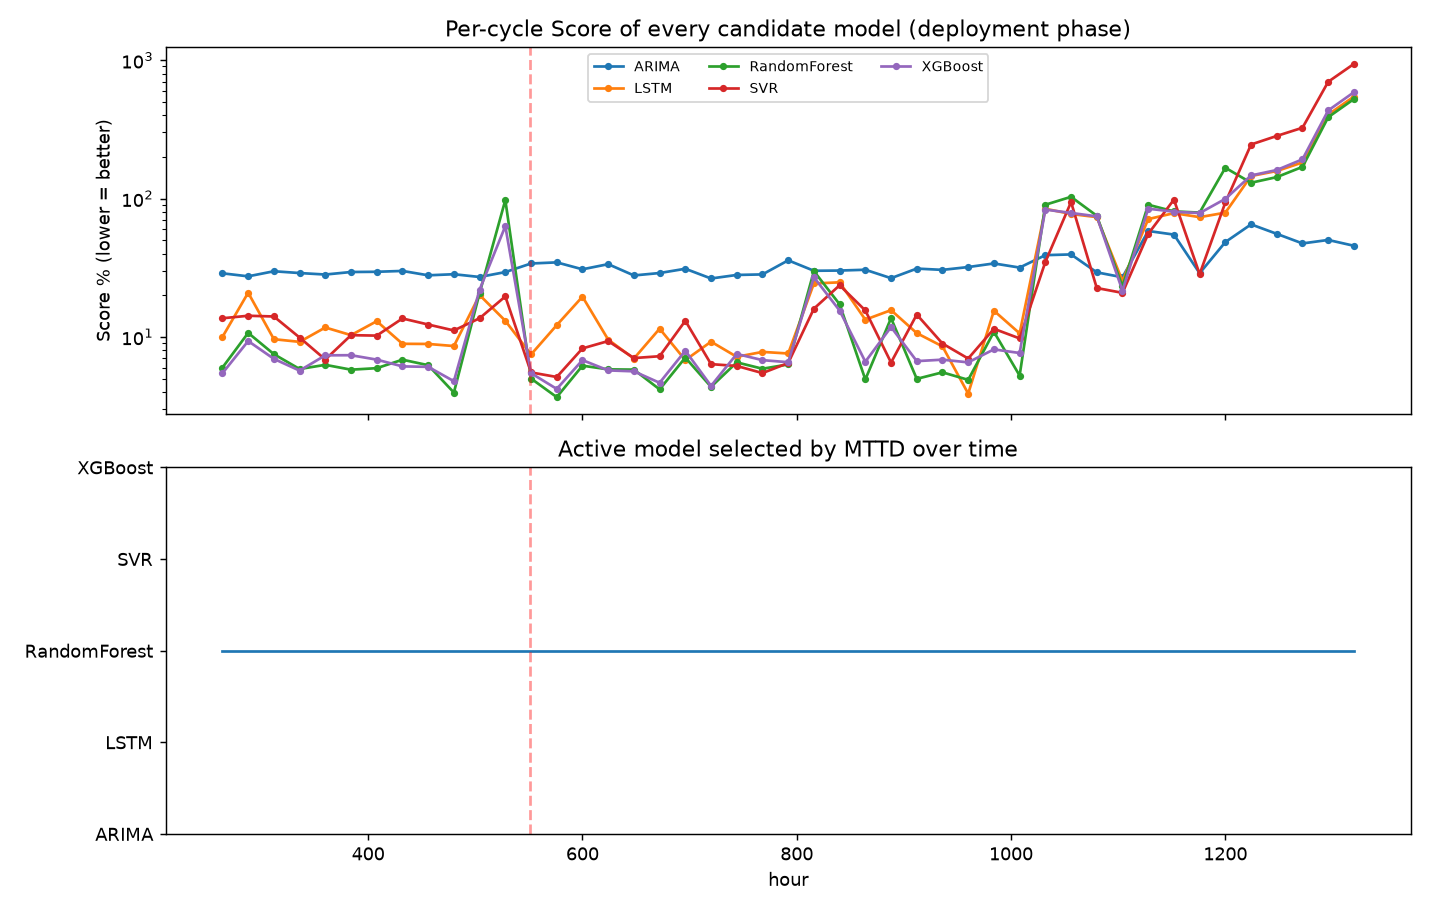
\includegraphics[width=0.85\linewidth]{fig5_all5.png}
\caption{Standard MTTD. Top: daily score of all five candidates (log scale). Bottom: active model; the dashed line marks the retraining event at hour 552.}
\label{fig:all5}
\end{figure}

\begin{table}[H]
\centering
\caption{Per-Candidate Accuracy in the Standard Run (1,080 Hours)}
\label{tab:permodel}
\footnotesize
\begin{tabular}{@{}lrrr@{}}
\toprule
Candidate & Overall Score\% & Cycles with lowest score & Hours active\\
\midrule
SVR & 22.41 & 10 & 0\\
LSTM & 29.72 & 3 & 0\\
ARIMA & 30.61 & 8 & 0\\
XGBoost & 30.66 & 10 & 0\\
Random Forest & 32.78 & 14 & 1,080\\
\bottomrule
\end{tabular}
\end{table}

\subsection{Periodic Reselection}
Table~\ref{tab:runs} compares the standard run with daily and hourly reselection. Figs.~\ref{fig:daily} and~\ref{fig:hourly} show the per-cycle scores and the active model over time, and Fig.~\ref{fig:fc} compares the forecasts with the actual load.

\begin{table}[H]
\centering
\caption{Forecast Accuracy of the Three MTTD Runs Over 1,080 Hours}
\label{tab:runs}
\footnotesize
\begin{tabularx}{\linewidth}{@{}l r r r r r L@{}}
\toprule
Run & Score\% & RMSE & MAE & Switches & Retrains & Hours active per model\\
\midrule
Standard MTTD & 32.78 & 13,649.96 & 5,945.88 & 0 & 1 (hour 552) & RF 1,080\\
Daily reselection & 21.41 & 8,412.83 & 4,239.58 & 27 & 0 & XGB 312, SVR 312, RF 168, LSTM 144, ARIMA 144\\
Hourly reselection & 18.96 & 7,757.50 & 3,536.08 & 77 & 1 (hour 864) & XGB 320, SVR 289, RF 235, LSTM 118, ARIMA 118\\
\bottomrule
\end{tabularx}
\end{table}

Daily reselection lowered the score by 34.7\% and hourly reselection by 42.2\% relative to standard MTTD, and both ended below the best single candidate of the standard run (SVR, 22.41\%). All five candidates were used in both runs. In the daily run the two-strike rule was never triggered, so no retraining took place; in the hourly run it triggered once, at hour 864, and the re-test selected Random Forest (6.78\%).

\begin{figure}[H]
\centering
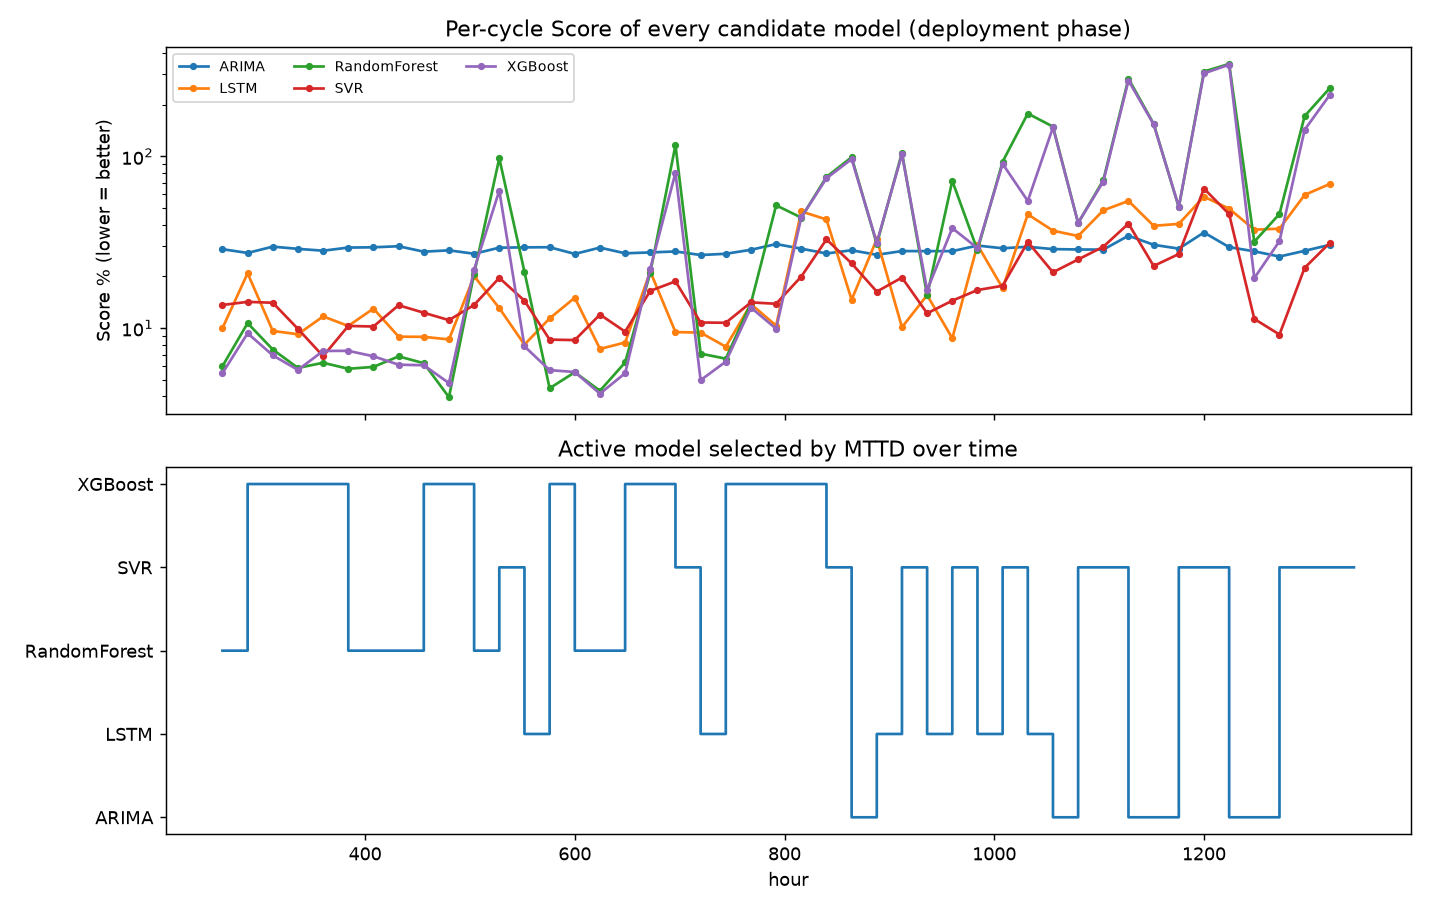
\includegraphics[width=0.85\linewidth]{fig_daily.png}
\caption{Daily reselection. Top: daily score of all five candidates. Bottom: active model over time (27 switches).}
\label{fig:daily}
\end{figure}

\begin{figure}[H]
\centering
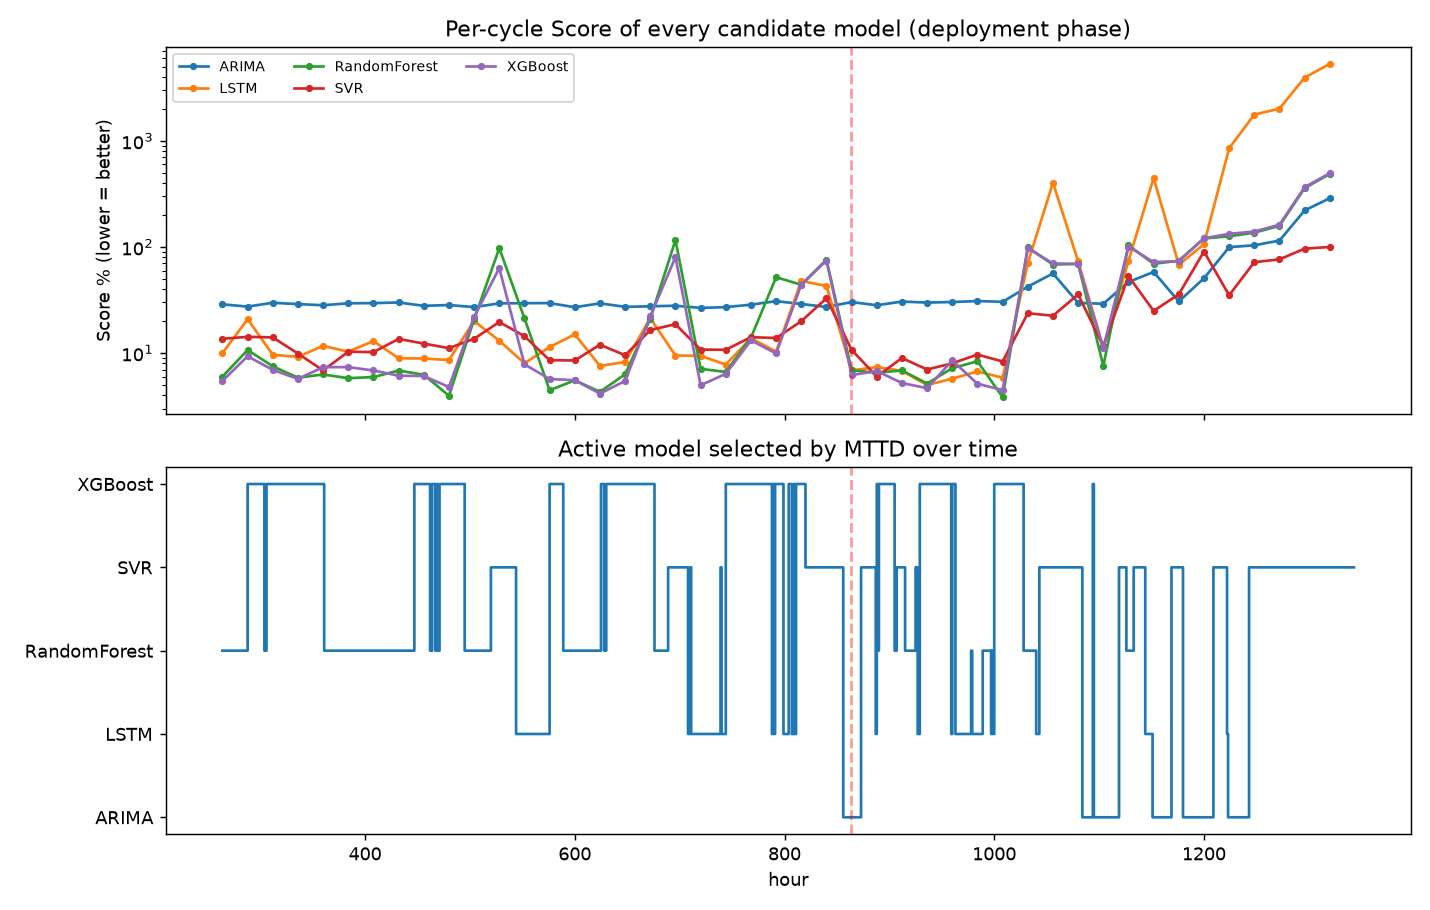
\includegraphics[width=0.85\linewidth]{fig_hourly.png}
\caption{Hourly reselection. Top: daily score of all five candidates. Bottom: active model over time (77 switches); the dashed line marks the retraining event at hour 864.}
\label{fig:hourly}
\end{figure}

\begin{figure}[H]
\centering
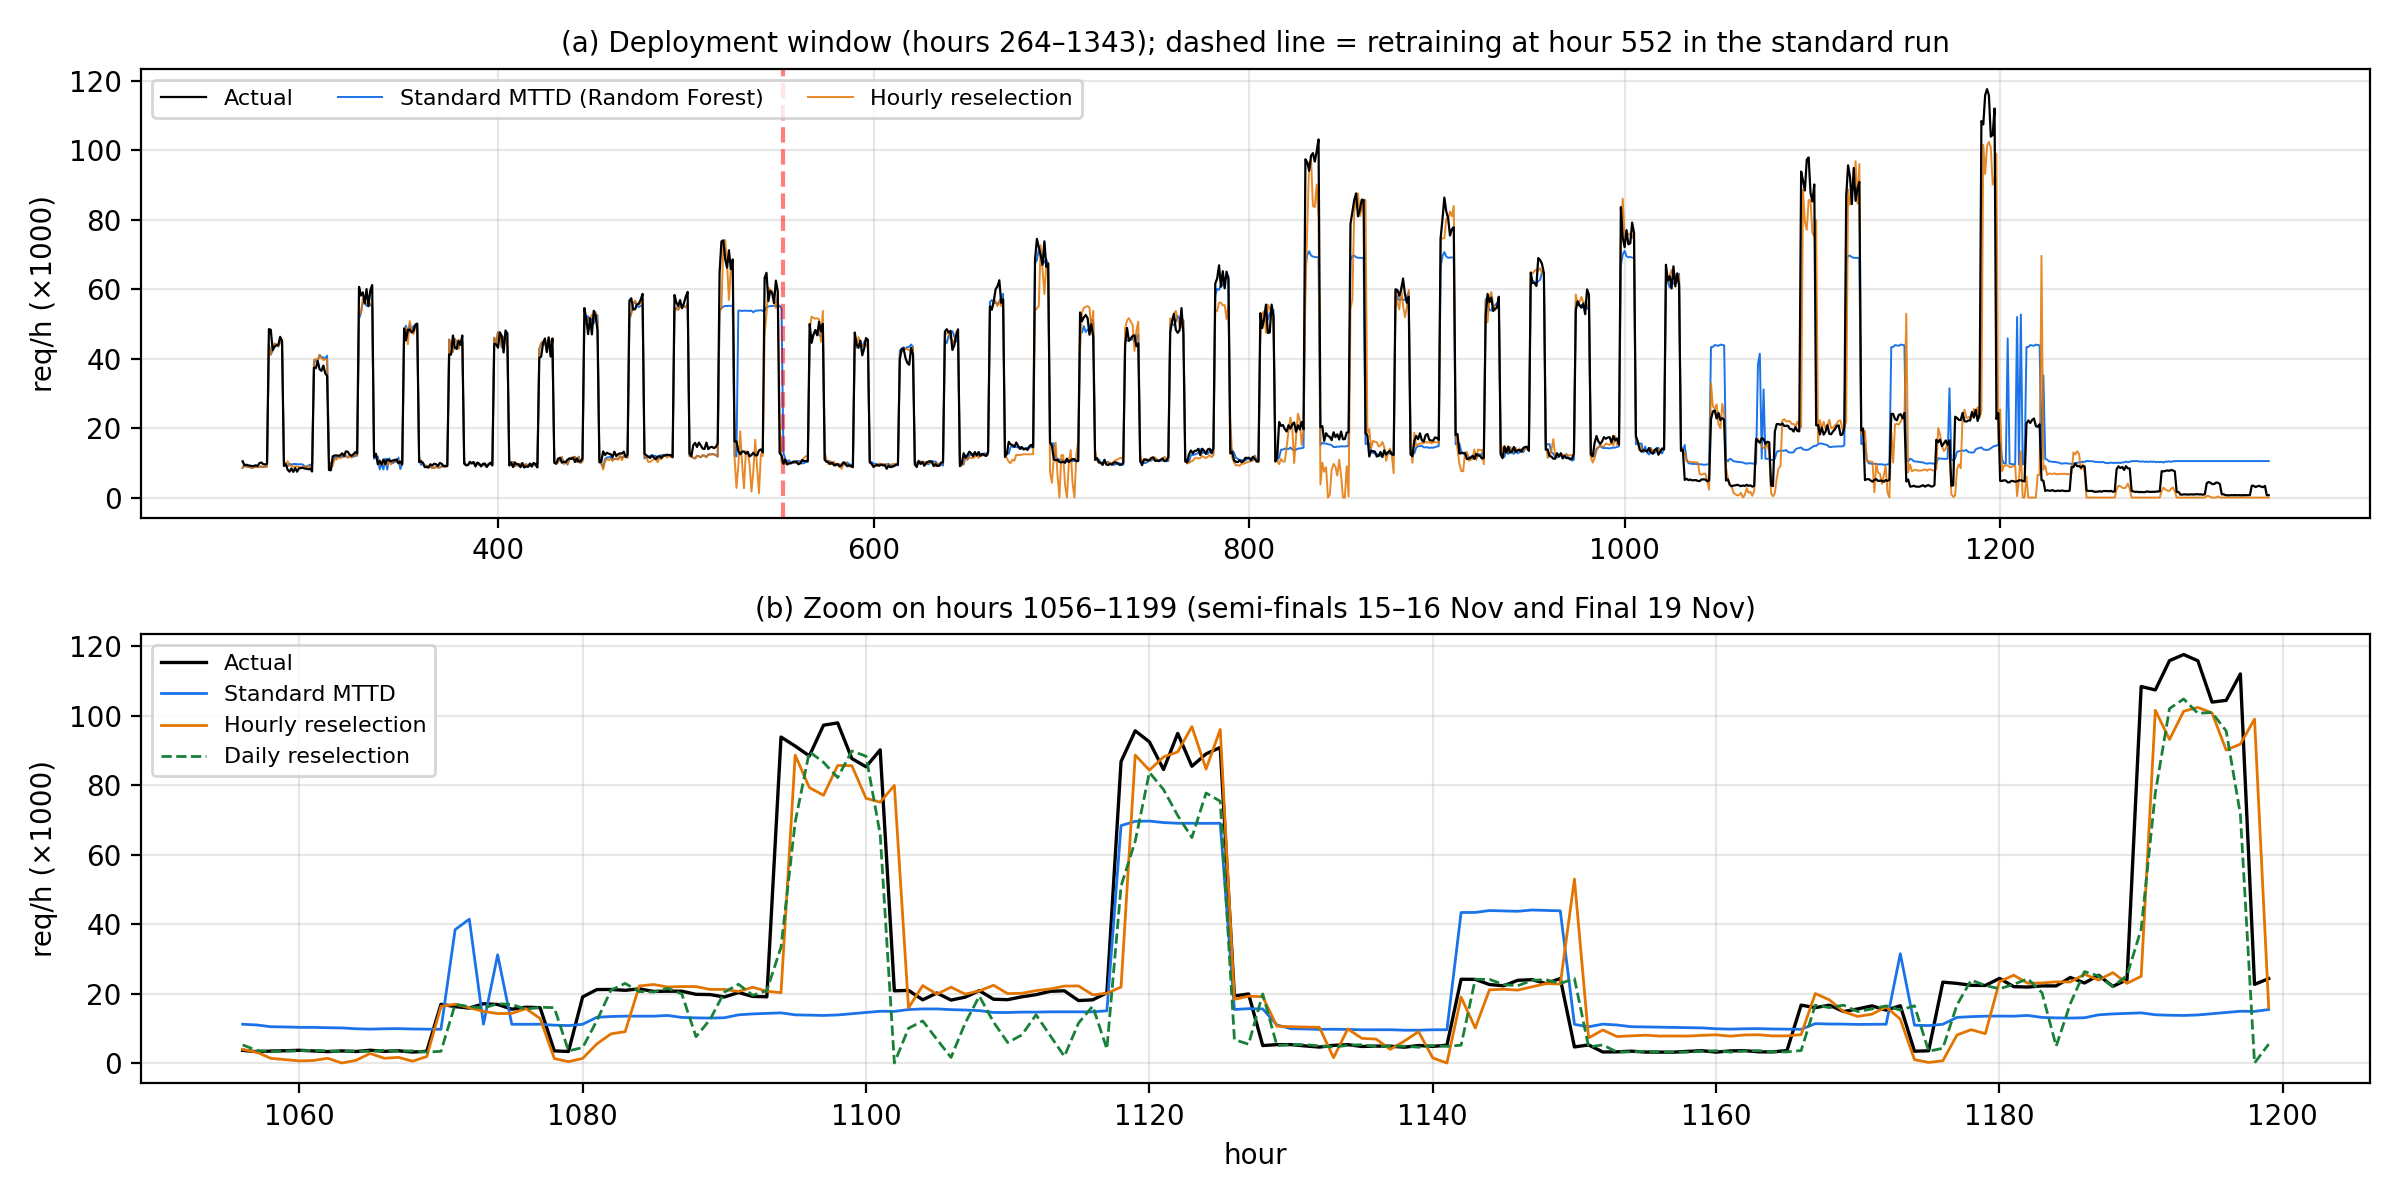
\includegraphics[width=\linewidth]{fig6_forecasts.png}
\caption{(a) Actual load and the forecasts of standard MTTD and hourly reselection over the deployment window. (b) Zoom on the semi-finals and the Final, including daily reselection.}
\label{fig:fc}
\end{figure}

\subsection{CloudSim Provisioning}
Each run's forecasts were replayed in CloudSim over the 1,080 deployment hours. Fig.~\ref{fig:console} shows the console output of the three simulations and Table~\ref{tab:cloudsim} and Fig.~\ref{fig:cs} summarise them. The same load was used in all three, so the VMs needed for the exact load total 6,981 VM-hours in each case.

\begin{figure}[H]
\centering
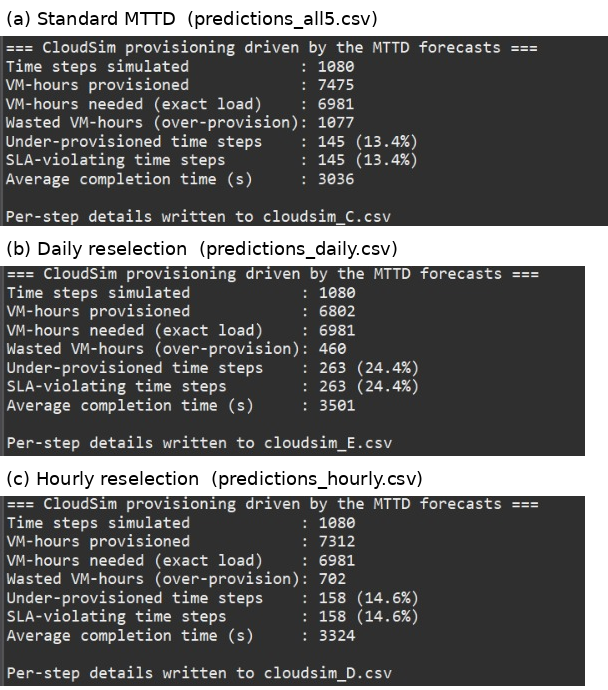
\includegraphics[width=0.75\linewidth]{fig8_cloudsim_summaries.png}
\caption{CloudSim 3.0.3 console output for (a) standard MTTD, (b) daily reselection and (c) hourly reselection.}
\label{fig:console}
\end{figure}

\begin{table}[H]
\centering
\caption{CloudSim Provisioning Results Over 1,080 Hours}
\label{tab:cloudsim}
\footnotesize
\begin{tabular}{@{}lrrrrr@{}}
\toprule
Run & VM-hours & Wasted VMh & Under-prov.\ hours & SLA-violating hours & Avg completion (s)\\
\midrule
Standard MTTD & 7,475 & 1,077 & 145 & 145 (13.4\%) & 3,036\\
Daily reselection & 6,802 & 460 & 263 & 263 (24.4\%) & 3,501\\
Hourly reselection & 7,312 & 702 & 158 & 158 (14.6\%) & 3,324\\
\midrule
Exact load (needed) & 6,981 & -- & -- & -- & --\\
\bottomrule
\end{tabular}
\end{table}

\begin{figure}[H]
\centering
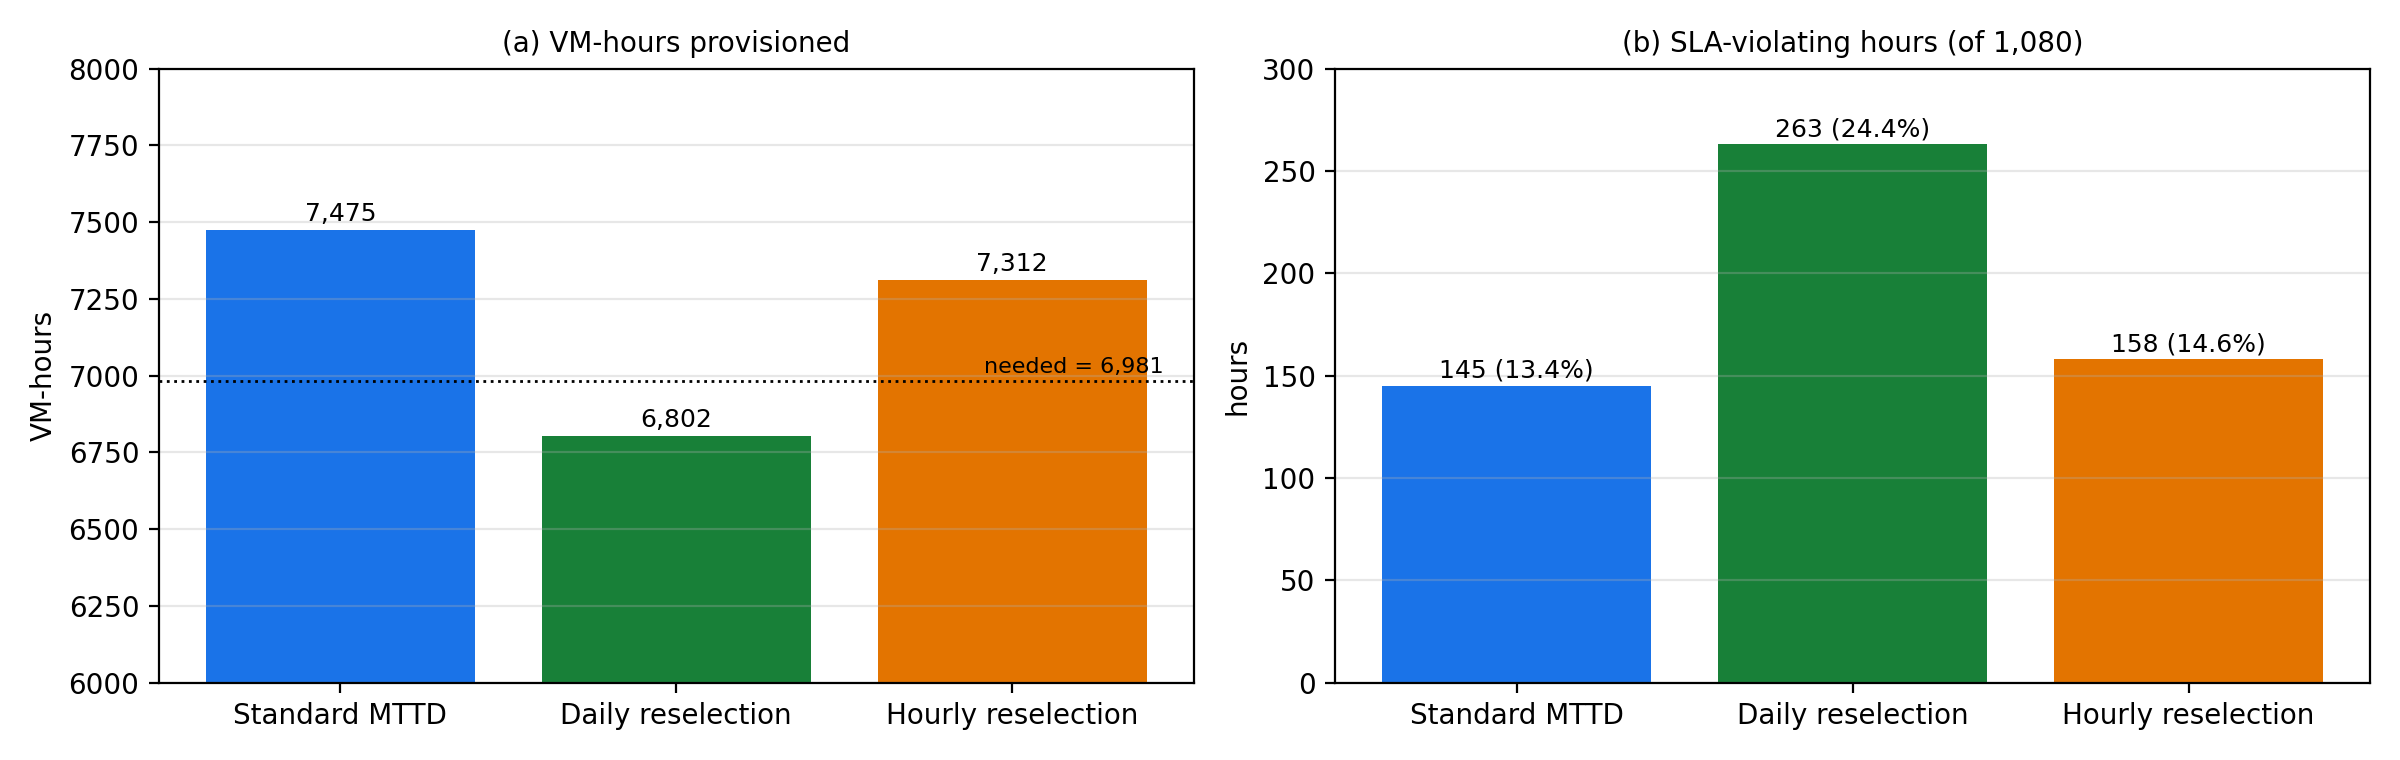
\includegraphics[width=0.95\linewidth]{fig9_cloudsim_runs.png}
\caption{(a) VM-hours provisioned by each run against the 6,981 VM-hours needed. (b) SLA-violating hours.}
\label{fig:cs}
\end{figure}

Standard MTTD provisioned 7.1\% more VM-hours than needed and violated the SLA in 145 hours. Hourly reselection provisioned 4.7\% more than needed, reduced wasted VM-hours by 34.8\% (702 vs.\ 1,077), and violated the SLA in 158 hours. Daily reselection provisioned 2.6\% fewer VM-hours than needed, reduced wasted VM-hours by 57.3\% (460), and violated the SLA in 263 hours. In every run each SLA-violating hour was an under-provisioned hour. The lower forecast error of the reselection runs therefore came with less over-provisioning but more hours in which the forecast was too low.

\subsection{Comparison with the Original Study}
On the synthetic patterns our reproduction agrees with~\cite{nashaat2026} that ARIMA performs well on the smooth uniform workload (the original reports a test-phase Score of 0.47\%, ours is 1.51\%), but differs on the random workload, where the original reports SVR as best. On the cricket trace, the pipeline behaved as designed: the test phase selected the lowest-scoring model, isolated bad cycles were absorbed, and two consecutive breaches triggered retraining and reselection. Because the active model changes only at retraining, Random Forest remained active even though the best-scoring model changed between cycles. Re-selecting periodically made both added models, XGBoost and the LSTM, active for part of the deployment; XGBoost was active for the most hours in the hourly run and, together with SVR, in the daily run.

\subsection{Threats to Validity}
\emph{Semi-synthetic data.} Only the daily totals are measured; the hourly shape, match window and noise are modelled. \emph{Proxy traffic.} Page views are not server requests and their burst statistics may differ from HTTP logs such as FIFA 1998~\cite{arlitt2000}. \emph{Single trace and seed.} Results come from one tournament, one noise seed and one train/test configuration. \emph{Cross-validation.} \texttt{GridSearchCV} with ordinary $k$-fold validation does not respect time order. \emph{Non-seasonal ARIMA.} ARIMA was run without a seasonal term. \emph{Simulation model.} VM capacity is fixed at 4,000 requests per hour; the simulation ignores VM start-up time and uses hour-long decision intervals.

\section{Conclusion and Future Work}\label{sec:conclusion}
We reproduced the MTTD framework of Nashaat \emph{et al.} with five candidate models instead of three and a 2023 Cricket World Cup workload instead of FIFA logs, and replayed its forecasts in CloudSim. In standard MTTD, Random Forest was selected at the test phase and again at the single retraining event, and remained active for all 1,080 hours with a score of 32.78\%, while the best-scoring model changed from cycle to cycle. Re-selecting the model every day or every hour made MTTD switch between all five candidates and lowered the score to 21.41\% and 18.96\%. In CloudSim, standard MTTD violated the SLA in 145 of 1,080 hours; hourly reselection reduced wasted VM-hours by 34.8\% but violated the SLA in 158 hours, and daily reselection in 263.

Future work includes validating on measured hourly or minute-level server logs of live sports events, reducing under-provisioning during sudden peaks, integrating MTTD forecasts with the Kubernetes Horizontal Pod Autoscaler~\cite{k8shpa}, and using multivariate inputs such as CPU, memory and network metrics.

\begin{thebibliography}{39}
\bibitem{nashaat2026} M. Nashaat \emph{et al.}, ``A dynamic machine learning approach for workload prediction in cloud environments,'' \emph{Sci. Rep.}, vol.~16, art. no. 10983, 2026, doi: 10.1038/s41598-026-40777-z.
\bibitem{calheiros2011} R. N. Calheiros, R. Ranjan, A. Beloglazov, C. A. F. De Rose, and R. Buyya, ``CloudSim: A toolkit for modeling and simulation of cloud computing environments and evaluation of resource provisioning algorithms,'' \emph{Softw. Pract. Exper.}, vol.~41, no.~1, pp.~23--50, 2011.
\bibitem{calheiros2015} R. N. Calheiros, E. Masoumi, R. Ranjan, and R. Buyya, ``Workload prediction using ARIMA model and its impact on cloud applications' QoS,'' \emph{IEEE Trans. Cloud Comput.}, vol.~3, no.~4, pp.~449--458, 2015.
\bibitem{box2015} G. E. P. Box, G. M. Jenkins, G. C. Reinsel, and G. M. Ljung, \emph{Time Series Analysis: Forecasting and Control}, 5th ed. Hoboken, NJ, USA: Wiley, 2015.
\bibitem{hyndman2008} R. J. Hyndman and Y. Khandakar, ``Automatic time series forecasting: The forecast package for R,'' \emph{J. Stat. Softw.}, vol.~27, no.~3, pp.~1--22, 2008.
\bibitem{drucker1997} H. Drucker, C. J. C. Burges, L. Kaufman, A. Smola, and V. Vapnik, ``Support vector regression machines,'' in \emph{Proc. NIPS}, 1997, pp.~155--161.
\bibitem{breiman2001} L. Breiman, ``Random forests,'' \emph{Mach. Learn.}, vol.~45, no.~1, pp.~5--32, 2001.
\bibitem{chen2016} T. Chen and C. Guestrin, ``XGBoost: A scalable tree boosting system,'' in \emph{Proc. 22nd ACM SIGKDD Int. Conf. Knowl. Discov. Data Min.}, 2016, pp.~785--794.
\bibitem{hochreiter1997} S. Hochreiter and J. Schmidhuber, ``Long short-term memory,'' \emph{Neural Comput.}, vol.~9, no.~8, pp.~1735--1780, 1997.
\bibitem{karim2021} M. E. Karim, M. M. S. Maswood, S. Das, and A. G. Alharbi, ``BHyPreC: A novel Bi-LSTM based hybrid recurrent neural network model to predict the CPU workload of cloud virtual machine,'' \emph{IEEE Access}, vol.~9, pp.~131476--131495, 2021.
\bibitem{lorido2014} T. Lorido-Botran, J. Miguel-Alonso, and J. A. Lozano, ``A review of auto-scaling techniques for elastic applications in cloud environments,'' \emph{J. Grid Comput.}, vol.~12, no.~4, pp.~559--592, 2014.
\bibitem{qu2018} C. Qu, R. N. Calheiros, and R. Buyya, ``Auto-scaling web applications in clouds: A taxonomy and survey,'' \emph{ACM Comput. Surv.}, vol.~51, no.~4, art. no. 73, 2018.
\bibitem{arlitt2000} M. Arlitt and T. Jin, ``A workload characterization study of the 1998 World Cup Web site,'' \emph{IEEE Netw.}, vol.~14, no.~3, pp.~30--37, 2000.
\bibitem{jung2002} J. Jung, B. Krishnamurthy, and M. Rabinovich, ``Flash crowds and denial of service attacks: Characterization and implications for CDNs and web sites,'' in \emph{Proc. 11th Int. World Wide Web Conf.}, 2002, pp.~293--304.
\bibitem{roy2011} N. Roy, A. Dubey, and A. Gokhale, ``Efficient autoscaling in the cloud using predictive models for workload forecasting,'' in \emph{Proc. IEEE 4th Int. Conf. Cloud Comput.}, 2011, pp.~500--507.
\bibitem{islam2012} S. Islam, J. Keung, K. Lee, and A. Liu, ``Empirical prediction models for adaptive resource provisioning in the cloud,'' \emph{Future Gener. Comput. Syst.}, vol.~28, no.~1, pp.~155--162, 2012.
\bibitem{gong2010} Z. Gong, X. Gu, and J. Wilkes, ``PRESS: PRedictive Elastic reSource Scaling for cloud systems,'' in \emph{Proc. Int. Conf. Netw. Serv. Manage. (CNSM)}, 2010, pp.~9--16.
\bibitem{shen2011} Z. Shen, S. Subbiah, X. Gu, and J. Wilkes, ``CloudScale: Elastic resource scaling for multi-tenant cloud systems,'' in \emph{Proc. 2nd ACM Symp. Cloud Comput.}, 2011, art. no. 5.
\bibitem{kim2016} I. K. Kim, W. Wang, Y. Qi, and M. Humphrey, ``Empirical evaluation of workload forecasting techniques for predictive cloud resource scaling,'' in \emph{Proc. IEEE 9th Int. Conf. Cloud Comput.}, 2016, pp.~1--10.
\bibitem{kim2022} I. K. Kim, W. Wang, Y. Qi, and M. Humphrey, ``Forecasting cloud application workloads with CloudInsight for predictive resource management,'' \emph{IEEE Trans. Cloud Comput.}, vol.~10, no.~3, pp.~1848--1863, 2022.
\bibitem{kumar2018} J. Kumar and A. K. Singh, ``Workload prediction in cloud using artificial neural network and adaptive differential evolution,'' \emph{Future Gener. Comput. Syst.}, vol.~81, pp.~41--52, 2018.
\bibitem{kumar2021} J. Kumar, A. K. Singh, and R. Buyya, ``Self directed learning based workload forecasting model for cloud resource management,'' \emph{Inf. Sci.}, vol.~543, pp.~345--366, 2021.
\bibitem{gao2020} J. Gao, H. Wang, and H. Shen, ``Machine learning based workload prediction in cloud computing,'' in \emph{Proc. 29th Int. Conf. Comput. Commun. Netw. (ICCCN)}, 2020, pp.~1--9.
\bibitem{bi2021} J. Bi, S. Li, H. Yuan, and M. Zhou, ``Integrated deep learning method for workload and resource prediction in cloud systems,'' \emph{Neurocomputing}, vol.~424, pp.~35--48, 2021.
\bibitem{liu2017} C. Liu, C. Liu, Y. Shang, S. Chen, B. Cheng, and J. Chen, ``An adaptive prediction approach based on workload pattern discrimination in the cloud,'' \emph{J. Netw. Comput. Appl.}, vol.~80, pp.~35--44, 2017.
\bibitem{cetinski2015} K. Cetinski and M. B. Juric, ``AME-WPC: Advanced model for efficient workload prediction in the cloud,'' \emph{J. Netw. Comput. Appl.}, vol.~55, pp.~191--201, 2015.
\bibitem{messias2016} V. R. Messias, J. C. Estrella, R. Ehlers, M. J. Santana, R. C. Santana, and S. Reiff-Marganiec, ``Combining time series prediction models using genetic algorithm to autoscale Web applications hosted in the cloud infrastructure,'' \emph{Neural Comput. Appl.}, vol.~27, no.~8, pp.~2383--2406, 2016.
\bibitem{amiri2017} M. Amiri and L. Mohammad-Khanli, ``Survey on prediction models of applications for resources provisioning in cloud,'' \emph{J. Netw. Comput. Appl.}, vol.~82, pp.~93--113, 2017.
\bibitem{masdari2020} M. Masdari and A. Khoshnevis, ``A survey and classification of the workload forecasting methods in cloud computing,'' \emph{Cluster Comput.}, vol.~23, no.~4, pp.~2399--2424, 2020.
\bibitem{moreno2019} R. Moreno-Vozmediano, R. S. Montero, E. Huedo, and I. M. Llorente, ``Efficient resource provisioning for elastic cloud services based on machine learning techniques,'' \emph{J. Cloud Comput.}, vol.~8, art. no. 5, 2019.
\bibitem{herbst2013} N. R. Herbst, S. Kounev, and R. Reussner, ``Elasticity in cloud computing: What it is, and what it is not,'' in \emph{Proc. 10th Int. Conf. Autonomic Comput. (ICAC)}, 2013, pp.~23--27.
\bibitem{rzadca2020} K. Rzadca \emph{et al.}, ``Autopilot: Workload autoscaling at Google,'' in \emph{Proc. 15th Eur. Conf. Comput. Syst. (EuroSys)}, 2020, art. no. 16.
\bibitem{verma2015} A. Verma, L. Pedrosa, M. Korupolu, D. Oppenheimer, E. Tune, and J. Wilkes, ``Large-scale cluster management at Google with Borg,'' in \emph{Proc. 10th Eur. Conf. Comput. Syst. (EuroSys)}, 2015, art. no. 18.
\bibitem{k8shpa} The Kubernetes Authors, ``Horizontal Pod Autoscaling,'' Kubernetes Documentation. [Online]. Available: \url{https://kubernetes.io/docs/tasks/run-application/horizontal-pod-autoscale/}
\enlargethispage{3\baselineskip}
\bibitem{gama2014} J. Gama, I. \v{Z}liobait\.{e}, A. Bifet, M. Pechenizkiy, and A. Bouchachia, ``A survey on concept drift adaptation,'' \emph{ACM Comput. Surv.}, vol.~46, no.~4, art. no. 44, 2014.
\bibitem{hyndman2006} R. J. Hyndman and A. B. Koehler, ``Another look at measures of forecast accuracy,'' \emph{Int. J. Forecast.}, vol.~22, no.~4, pp.~679--688, 2006.
\bibitem{pedregosa2011} F. Pedregosa \emph{et al.}, ``Scikit-learn: Machine learning in Python,'' \emph{J. Mach. Learn. Res.}, vol.~12, pp.~2825--2830, 2011.
\bibitem{paszke2019} A. Paszke \emph{et al.}, ``PyTorch: An imperative style, high-performance deep learning library,'' in \emph{Proc. Adv. Neural Inf. Process. Syst. (NeurIPS)}, 2019, pp.~8024--8035.
\bibitem{wikimedia} Wikimedia Foundation, ``Wikimedia REST API: Pageviews per-article endpoint.'' [Online]. Available: \url{https://wikimedia.org/api/rest_v1/}
\end{thebibliography}
\end{document}
